\newpage\chapter{Introduzione alla farmacologia}

\section{Definizioni generali}

\begin{description}

\item[Farmacologia] lo studio di sostanze che interagiscono con gli esseri vivnti con processi chimici, con molecole regolatrici e attraverso l'attivazione ol'inibizione di normali processi organici.

\item[Farmacologia medica] scienza che si occupa delle sostanze utilizzate per prevenire, diagnosticare e trattale le malattie

\item[Tossicologia] branca della farmacologia che si occupa degli effetti dannosi delle sostanze chimiche sui viventi

\item[Farmacogenomica] studio delle variazioni genetiche che causano differenze individuali nella risposta ai farmaci

\item[Farmaco] qualsiasi sostanza in grado di indurre, attraverso le sue azioni chimiche, modifiche di funzioni biologiche


\item[Recettore] molecola biologica che svolge un ruolo regolatorio.

\end{description}

\begin{tikzpicture}
	\Tree
	[.{Farmaco agisce}
		[.{sui recettori}
			{come agonista (attivatore)}
			{come antagonista (inibitore)}
		]
		[.{non mediata\\ da recettori}
			{agenti osmotici\\(mannitolo nei tubuli)}
			{interazione chimica diretta\\(antiacidi)}
		]
		[.{con altri farmaci}
			{come agonista o\\ antagonista chimico}
		]
	]
\end{tikzpicture}

\begin{tikzpicture}
	\Tree
	[.{Fisicamente è}
		{solido (aspirina, atropina...)}
		{liquido (nicotina, etanolo...)}
		{gas (protossido d'azoto)}
	]
\end{tikzpicture}

\begin{tikzpicture}
	\Tree
	[.{Composto da}
		carboidrati
		proteine
		lipidi
	]
\end{tikzpicture}

Dimensione da 7pm (litio) a 59000pm (alteplase) ma usualmente compreso da 100 a 1000pm.

\begin{description}

\item[Farmacodinamica] Definisce le azioni di un farmaco sull'organismo e le relazioni tra concentrazione e effetto.

\item[Farmacocinetica] Definisce le azioni dell'organismo sul farmaco e le relazioni tra dose e concentrazione, l'assorbimento, la distribuzione e l'eliminazione del farmaco

\item[Molecola effettrice/effettore] molecola che attiva la modifica funzionare finale. Può essere parte del recettore o una molecola separata.
\end{description}

Un farmaco (F) agisce su un recettore R attivando (*) un effettore (E) o passando per una molecola accoppiante (G) secondo una di queste tappe

\begin{eqnarray*}
F + R \longrightarrow FR + E \longrightarrow FRE^* \longrightarrow\text{effetto}\\
F + R \longrightarrow FR + E \longrightarrow E^* \longrightarrow\text{effetto} \\
F + R \longrightarrow FR + G \longrightarrow G^* + E \longrightarrow E^*  \longrightarrow\text{effetto}
\end{eqnarray*}

L'inibizione del metabolismo di un attivatore endogeno porta a \upa attivatore e quindi \upa effetto.

\begin{tikzpicture}
	\Tree
	[.{Interazione\\ farmaco\\ recettore}
		[.agonista
			{si lega al sito di legame e\\ attiva la funzione dell'agonista}
		]
		[.antagonista
			{si lega al sito di legame\\ impedendo la funzione dell'agonista}
		]
		[.{allosterico\\(su altro sito)}
			[.attivatore
				{aumenta la funzione dell'agonista}
			]
			[.inibitore
				{diminuisce la funzione dell'agonista}
			]
		]
	]
\end{tikzpicture}

Un recettore R senza agonisti vive normalmente in un equilibro fra la sua forma inattivata $R_I$ preferenziale e la sua forma attivata $R_A$. Quindi, anche senza agonista ha una sua attività di base detta \textbf{attività costitutiva}.

Un farmaco agonista sposta l'equilibrio verso $R_A$

\begin{eqnarray*}
\schemestart $R_I$\arrow{<<->}$R_A$ \schemestop \\
\schemestart $R_I + F$\arrow{<->>}$R_A + F$ \schemestop
\end{eqnarray*}

\begin{description}
\item[Agonisti pieni] quei farmaci che danno viraggio quasi completo di $R$ nella forma $R_A$
\item[Agonisti parziali] non stabilizzano la forma $R_A$ in modo completo. Questi, se presente un agonista pieno, si comportano da antagonisti nei confronti di quello pieno.
\item[Antagonista (neutro)] farmaco che blocca l'accesso al recettore prevenendone l'effetto ma ininfluente sull'equilibrio dello stato $R_I$
\item[Agonista inverso]farmaco che stabilizza lo stato $R_I$ diminuendo l'attività costitutiva del recettore
\end{description}

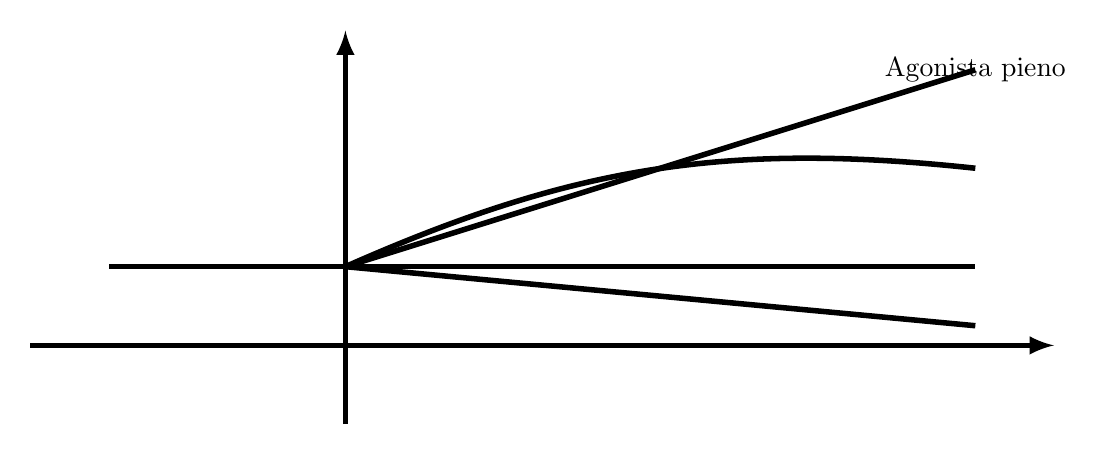
\begin{tikzpicture}
	\tikzstyle{none}=[inner sep=0pt]
	\tikzstyle{arrow1}=[-latex,draw,line width=2.000]
	\tikzstyle{simple}=[-,draw,line width=2.000]
		\node [style=none] (0) at (0, 4) {};
		\node [style=none] (1) at (9, -0) {};
		\node [style=none] (2) at (0, -1) {};
		\node [style=none] (3) at (-4, -0) {};
		\node [style=none] (4) at (-3, 1) {};
		\node [style=none] (5) at (0, 1) {};
		\node [style=none] (6) at (8, 3.5) {Agonista pieno};
		\node [style=none] (7) at (8, 2.25) {};
		\node [style=none] (8) at (8, 1) {};
		\node [style=none] (9) at (8, 0.25) {};

		\draw [style=arrow1] (3.center) to (1.center);
		\draw [style=arrow1, in=-90, out=90, looseness=1.00] (2.center) to (0.center);
		\draw [style=simple] (4.center) to (5.center);
		\draw [style=simple] (5.center) to (6.center);
		\draw [style=simple, bend left=15, looseness=1.00] (5.center) to (7.center);
		\draw [style=simple] (5.center) to (8.center);
		\draw [style=simple] (5.center) to (9.center);

\end{tikzpicture}

\begin{tikzpicture}
	\tikzset{level 3/.style={level distance=130pt}}
	\Tree
	[.{Meccanismo di diffusione}
		[.{verso il sito}
			[.{acquosa via}
				citosol
				{spazio interstiziale}
				{giunzioni serrate}
			]
			trasportatori
			endocitosi
			esocitosi
		]
		[.{fuori dal sito}
			[.{ABC\\(ATP binding cassette}
				{MPR\\(nel cervello, testicoli)}
				{MDR1\\(multidrug resistence proteine\\ nelle neoplasie)}
			]
		]
	]
\end{tikzpicture}

\begin{description}
\item[Legge di Fick]
$$ \Phi_{n.mol/s} = \Delta C \cdot \frac{S\cdot C_p}{d} \qquad\text{dove}$$

$\Delta C = C_1 - C_2$ differenza di concentrazione con $C_1 > C_2$\newline
$S$ area di diffusione\newline
$d$ spessore della via di diffusione\newline
$C_p$ coefficiente di diffusione

\item[Acido debole] molecola neutra che può reversibilmente dissociarsi in un anione 

$$\ce{HA <-> A- + H+}$$

\item[Base debole] molecola neutra che può reversibilmente formare un catione

$$\ce{BH+ <-> B + H+}$$

Poichè la diffusione lipidica è ostacolata dalla ionizzazione allora un acido debole ha diffusione lipidica in forma protonata mentre la base debole ha diffusione lipidica nella forma non protonata.

\end{description}

\section{Eq. di Hasselback}

Definisce il rapporto tra forma protonata e non sulla base della costante di dissociazione \ce{pK_a} della sostanza e il \ce{pH} dell'ambiente ove il \ce{pK_a} è il \ce{pH} ove \ce{[HA] = [A-]} e tale che

$$\log\frac{\ce{[HA]}}{\ce{[A^-]}} = \ce{pK_a} - \ce{pH}$$

che si applica sia alle basi che agli acidi deboli. Per cui a $\ce{pH} > \ce{pK_a}$ si avrà che quella più rappresentata è la forma deprotonata ossia quella lipofilica per le basi deboli mentre a $\ce{pH} < \ce{pK_a}$ quella più rappresentata sarà quella protonata ossia la forma lipofilica per gli acidi deboli.

L'uso dell'eq. di Hasselback può essere molto utile qualora si desideri causare intrappolamento o riassorbimeno di un farmaco nello stomaco, nell'intestino, latte materno, secrezioni prostatiche, vaginali e/o apparato urinario.

Ad esempio se si vuole accellerare l'escrezione di una metanfetamina, base debole $\ce{pK_a} = 10$ per via urinaria bisogna impedirne il riassorbimento. Acidificando le urine con cloruro di ammonio si ottiene un equilibrio spostato verso la forma protonata che, nelle basi deboli, è la forma ionizzata e quindi lipofobica impedendone il riassorbimento dalle pareti dei tuboli renali.

\section{Eq. legame agonista--recettore}

Supponendo una interazione all'equilibro tra farmaco F e recettore R del tipo

$$ \ce{R + F <->[K_1][K_{-1}] RF} $$

si ha che $\Delta[RF] = K_1[R][F] - K_{-1}[RF]$ che, all'equilibrio è uguale a zero da cui

$K_{-1}[RF] = K_1[R][F]$ e, d'altra parte, la concentrazione di farmaco totale è uguale a quello non legato sommato a quello legato quindi

$F_{Tot} = [R] + [RF] \Rightarrow [R] = F_{Tot} - [RF]$ e sostituito

$K_{-1}[RF] = K_1[F](F_{tot} - [RF]) = K_1[F]F_{Tot} - K_1[F][RF]$ e raccogliendo

$[RF](K_{-1} + K_1[F]) = K_1F_T[F]$ da cui

$$[RF] = \frac{K_1F_T[F]}{K_{-1}+K_1[F]}=\frac{F_T[F]}{\frac{K_1}{K_1} + [F]}$$

e chiamando $K_d = \frac{K_1}{K_1}$ costante di dissociazione si ha che

$$[RF]=\frac{F_T\cdot[F]}{K_d+[F]}$$

Quindi la concentrazione del farmaco legato ai recettori dipende dalla concentrazione del farmaco libero $[F]$, da $F_T$ e da $K_d$.

$K_d$ indica l'affinità inversa del farmaco al recettore e quindi più $K_d$ è bassa maggiore è l'affinità. $K_d$ indica la concentrazione del farmaco che da 1/2 del farma max legato infatti ponendo $K_d =[F]$

$$ [RF] = \frac{F_T\cdot[F]}{2[F]}=\frac 12 F_T$$

Quando $[F]\rightarrow\infty, [RF] \rightarrow F_T$ quindi $F_T$ è la concentrazione di farmaco legato per concentrazioni di farmaco libero infinitamente alte.

Analoga relazione vi è tra l'effetto di un farmaco e la sua concentrazione

$$E =\frac{E_{max}\cdot[F]}{EC_{50} + F}$$

dove $E_{max}$ è l'effetto massimo ottenibile e $EC_{50}$ è la concentrazione del farmaco che da $\frac12 E_{max}$.

Spesso $K_d\simeq EC_{50}$ a causa dei recettori di riserva ossia si ottiene un effetto max con concentrazioni di agosnista molto minori di quelle supposte. Il motivo è dovuto al fatto che un singolo recettore attiva più di una singola risposta e questo è dato dal fatto che se io aggiungo piccole quantità di antagonista la curva di effetto si sposta verso destra ma $E_{max}$ rimane invariata perchè vengono reclutati nuovi recettori tra quelli di riserva. 

$EC_{50} \rightarrow K_d$ solo quando l'antagonista mi blocca quasi tutti i recettori di riserva e, da quel momento, anche $E_{max}$ inizia a diminuire.

Un antagonista competitivo a fronte di una concentrazione fissa $[I]$ dell'agonista produce un effetto ridotto $C'$ tale che, a parità di effetto

$$\frac{C'}{C} = 1+ \frac{[I]}{K'_D}$$

dove $K'_D$ è la costante di dissociazione dell'antagonista. 

Ma, come si nota, per $[I]\rightarrow\infty, \frac{C'}{C}\rightarrow 1$ infatti l'antagonista competitivo non alterà l'$E_{max}$ ma sposta solo la curva più a destra.

Nel caso invece di antagonisti irreversibili la perdità irreversibile di recettori può dar luogo a una diminuzione di $E_{max}$.

Altri due tipi di antagonismo sono:

\begin{description}
\item[Antagonismo chimico] un farmaco si lega ad un altro farmaco e lo neutralizza (antidoto). Ad esempio il \index{dimercaprolo}dimercaprolo, chelante del piombo.
\item[Antagonismo fisiologico] Un farmaco che agisce su recettori differenti dal primo ma con effetti opposti. Ad esempio i glucocorticoidi \upa glicemia. Si da allora insulina che \dwa glicemia. Un altro antagonismo fisiologico è l'adrenalina che broncodilata e anatagonizza l'azione broncocostrittrice dell'istamina.
\end{description}

\begin{description}
\item[Potenza farmacologica] relativa alla concentrazione $EC_{50}$ o alla dose $ED_{50}$ che causa il 50\% della risposta massima. Un farmaco è tanto più potente quanto più è bassa la $EC_{50}$, $ED_{50}$.

\item[Efficacia massima] E' la $E_{max}$ ossia la risposta massima che posso produrre indipendentemente dalla dose.
\end{description}

I concetti dose--risposta finora espressi sono basati su misure ex--vivo. Nell'essere umano le risposte invece dipendono da molteplici effetti.

Nel vivente si parla quindi di \textbf{curve quantali} ossia curve dose--effetto basate sull'integrale della gaussiana delle percentuali di individui che, ad una certa dose, ottengono un determinato effetto.

Queste percentuali si distribuiscono come una gaussiana attorno ad un valore medio che sarà detto $ED_{50}^m$ \textbf{dose efficace mediana} che causa l'effetto nel 50\% degli individui.

Se l'effetto misurato è una tossicità allora si parla di $TD_{50}^m$ \textbf{dose tossica mediana}. Se l'effetto misurato è la morte si parla di $LD_{50}^m$ dose letale mediana

{grafico}

\section{Indice terapeoutico o finestra terapeutica}

\`E una misura di quando "sicuro" sia un farmaco in quanto mette in relazione $TD_{50}^m$ con $ED_{50}^m$. Se questi valori sono simili, sono vicene le dosi efficaci con quelle tossiche e quindi il rischio tossicità è alto. Se lontane il farmaco è più sicuro

$$I_T=\frac{TD_{50}}{ED_{50}}$$

Ovviamente questo indice è dipendente dall'uso. Un farmaco per la cefalea deve avere un bassissimo rischio di tossicità mentre in uno per il linfoma di Hodking posso accettare anche un rischio di tossicità elevato in quanto il non trattamento porta alla morte.

\begin{tikzpicture}
	\Tree
	[.{Risposta individuale\\ ad un famaco}
		{nella norma}
		[.{iporeattivo}
			{effetto sotto $ED_{50}^m$}
		]
		[.{iperattivo}
			{effetto sopra $ED_{50}^m$}
		]
		[.{tolleranza}
			{risposta descresce dopo\\ somministrazioni ripetute}
		]
		[.{tachifilassi}
			{risposta descresce molto\\ rapidamente}
		]
		[.{idiosincrasica}
			{risposta insolita non\\ osservata nella maggior\\ parte dei pazienti}
		]
	]
\end{tikzpicture}

\begin{tikzpicture}
	\tikzset{level distance=150pt}
	\Tree
	[.{cause di variabilità\\ nelle risposte}
		{variazioni nella concentrazione}
		{di farmaco che raggiunge il recettore}
		[.{variazione nel numero di recettori}
			{down--regolazione}
			{desensibilizzazione}
			{overshoot (rimbalzo\\ quando si interrompe\\ una cura}
		]
		{variazione nei componenti post--recettoriali}
		{variazione nella concentrazione di un liqido endogeno}
	]
\end{tikzpicture}

\begin{tikzpicture}
	\tikzset{level 2/.style={level distance=150pt}}
	\Tree
	[.{Cause di tossicità}
		[.{effetti terapeutici e tossici\\ mediati dallo stesso recettore}
			{sanguinamento da terapia anticoagulante}
			{ipoglicemia da insulina esogena}
		]
		[.{come sopra ma collegati\\ a effettori differenti}
			{glicosidi digitalici}
			{metrotrexato}
		]
		[.{mediato da recettori differenti}
			{farmaci aspecifici si legano a\\ diversi recettori con effetti diversi}
		]
	]
\end{tikzpicture}







